\documentclass[11pt,a4paper]{article}

\usepackage[pdftex]{graphicx}
\usepackage[cmex10]{amsmath}
\usepackage[usenames,dvipsnames]{color}
\usepackage{xspace}
\usepackage{fullpage}
\usepackage{tikz}
\usepackage{pgfplots}
\usepackage{pgfplotstable}
\usepackage{textcomp}
\usepackage{multirow}
\usetikzlibrary{shapes,arrows}
\usetikzlibrary{pgfplots.groupplots}
\usepackage{url}
\usepackage{listings}
\usepackage{framed}

\newcommand{\todo}[1]{\textbf{\textcolor{Blue}{TODO: #1}}}
\newcommand{\lst}[1]{\lstinline!#1!}
\newcommand{\fig}[1]{Fig.~\ref{#1}}
\newcommand{\eq}[1]{(\ref{#1})}
\newcommand{\ap}[1]{Appendix~\ref{#1}}
\newcommand{\tbl}[1]{Tbl.~\ref{#1}}
\newcommand{\file}[1]{\lstinline[basicstyle=\normalsize,]!#1!}
\newcommand{\pder}[2]{\frac{\partial{#1}}{\partial{#2}}}
\newcommand{\neuron}{CoreBluron}
\newcommand{\dx}{{\Delta x}}
\newcommand{\dt}{{\Delta t}}
\newcommand{\at}[1]{{#1}_{i}}
\newcommand{\atplus}[1]{{#1}_{i+1}}
\newcommand{\atminus}[1]{{#1}_{i-1}}
\newcommand{\atplushalf}[1]{{#1}_{i+\frac{1}{2}}}
\newcommand{\atminushalf}[1]{{#1}_{i-\frac{1}{2}}}
\newcommand{\vv}[1]{\mathbf{#1}}
\newcommand{\att}[1]{{#1}^{n}}
\newcommand{\attplus}[1]{{#1}^{n+1}}
\newcommand{\attplushalf}[1]{{#1}^{n+\frac{1}{2}}}

\lstdefinelanguage{julia}
{
    morekeywords = {
        if, elseif, else,
        for, while, end, in, using,
        type, function, return, yieldto, try, catch, error, throw, begin, quote,
        Int, Int32, Int64, Float, Float32, Float64, Array
    },
    sensitive = true,
    morecomment=[l]\#,
    morestring=[b]",
    morestring=[b]',
    moredelim=*[directive]@,
    moredirectives={assert, time, eval} % macros
}[keywords,comments,strings,directives]


\lstset{
    language=[ANSI]C++,
    %numbers=left,
    basicstyle=\small\ttfamily,
    identifierstyle=\color{Blue}\small\ttfamily,
    keywordstyle=\color{Red}\small\ttfamily\bf,
    commentstyle=\color{OliveGreen}\small\ttfamily
}

\definecolor{shadecolor}{rgb}{0.8,0.8,0.8}

\begin{document}

% title and cover page
\title{CoreBluron Overview}
\author{Ben Cumming\\CSCS -- Swiss National Supercomputing Center}
\date{\today}
\maketitle

% abstract
\abstract{
This document presents an overview of the CoreBluron code that was released as part of the PCP process for the Human Brain Project in July 2014. The analysis reguards the code from a computational intensity point of view. That is, the focus is to describe the structure of the code that has the highest computational overheads.

More detailed analysis of the algorithms themselves, and important parts of the code like spike communication, that do not dominate the time to solution in the benchmarks available for this analysis. For now I will focus on just the computationally intensive parts of the code.
}

%%%%%%%%%%%%%%%%%%%%%%%%%%%%%%%%%%%%%%%%%%%%%%%%%%%%%%%%%%%%%%
\section{Overview}
%%%%%%%%%%%%%%%%%%%%%%%%%%%%%%%%%%%%%%%%%%%%%%%%%%%%%%%%%%%%%%
The version of CoreBluron that was released for the PCP is derived directly from Bluron, a flavour of Neuron maintained by the Blue Brain Project (BBP) group at EPFL. CoreBluron is derived directly in the sense that it is a subset of the features and corresponding code from Bluron. The code has been modified as much as needed to remove it from the larger Bluron infrastructure, and reduce the memory footprint of the code.

%%%%%%%%%%%%%%%%%%%%%%%%%%%%%%%%%%%%%%%%%%%%%%%%%%%%%%%%%%%%%%
\section{The Code}
%%%%%%%%%%%%%%%%%%%%%%%%%%%%%%%%%%%%%%%%%%%%%%%%%%%%%%%%%%%%%%
The code in its current form is a mixture of C and C++.


It must be noted that the code base is currently very challenging to understand and benchmark. It is derived directly from the Bluron/Neuron code base. This is an old code base, that has grown organically over a period of more tha 20 years. As such there are very many opportunities to simplify and improve the code using modern programming languages and development techniqies.

To use both CPUs and accelerators (e.g. GPU and MIC) effectively, parts of the code will have to be refactored, or rewritten significantly. Rewriting will be challenging, given the difficulty of understanding the current code, which is a prerequisite for rewriting the code. Developing documentation of the algorithms as they are currently implemented is essential if the code is to be refactored.

From early work with the code base, the majority of wall time for the example circuits release for the PCP is spent in a relatively small set of code: the \lst{nrnoc} solver implementation, and the mechanisms defined in \lst{/mecb/cfiles}. The code in its current form might be quite complicated, however the algorithms themselves are relatively straightfoward.

An aim of this report is as a first attempt at describing the algorithms clearly, to make it possible to reason about how them without getting bogged down with the code.

%-------------------------------------------------------------
\subsection{Code Issues}
%-------------------------------------------------------------
Some of the anti-patterns that make understanding the code difficult are:
\begin{itemize}
    \item
        There are many global variables. With many static symbols used for scoping within a translation units, which makes understanding where variables are defined and used challenging.
    \item
        The use of preprocessor \lst{#define} makes the code very difficult to reason about. Many variable names are redefined, which obscures the meaning of the code. There are also many ``magic numbers'' that are defined on differently in different translation units.
    \item
        The C++ code uses new and delete keywords, sometimes forgetting to delete. Should use static arrays or STL containers depending on needs.
    \item
        overly complicated data structures that make it very difficult for both humans and compilers to reason about the code. As a result there are a lot of lost opportunities for optimization for the compiler.
    \item
        Poor (non-existant in places) comments and naming of variables.
\end{itemize}

%-------------------------------------------------------------
\subsection{Code Layout}
%-------------------------------------------------------------
The source code is packaged in a file \lst{CoreBluron.tar.gz}, which has the directory structure in \fig{fig:DirectoryStructure}.

In terms of time to solution, functions defined in \lst{mech/cfiles} dominate. These are called from the solver routines in \lst{nrnoc}, which implements the core computation, and has been to date the focus of my analysis.

\begin{figure}[tp!]
%---------------------------
\fbox{ \parbox{\textwidth} {

\begin{itemize}
    %%%%%%%%%%%%%%%%%%%%%%%%%%%%%%%%%%%%%%%%%
    \item \textbf{nrniv}
    \begin{itemize}
        \item C and C++ (11,470 lines).
        \item The \neuron driver: \lst{main()} is in \lst{main1.cpp}.
    \end{itemize}

    %%%%%%%%%%%%%%%%%%%%%%%%%%%%%%%%%%%%%%%%%
    \item \textbf{nrnoc}
    \begin{itemize}
        \item C (2,889 lines).
        \item The CoreBluron ``engine''
        \begin{itemize}
            \item storage
            \item solvers
            \item time stepping
            \item etc...
        \end{itemize}
    \end{itemize}

    %%%%%%%%%%%%%%%%%%%%%%%%%%%%%%%%%%%%%%%%%
    \item \textbf{mech/cfiles}
    \begin{itemize}
        \item C (11,301 lines).
        \item Definitions of all the mechanisms.
        \item generated from \lst{.hoc} files by Neuron.
        \item the generated code is very messy (use \lst{clang-format} to make things bearable)
    \end{itemize}

    %%%%%%%%%%%%%%%%%%%%%%%%%%%%%%%%%%%%%%%%%
    \item \textbf{nrnmpi}
    \begin{itemize}
        \item C (1,096 lines).
        \item Wrappers around MPI routines.
        \item Spike exchange implementation.
        \item Global variables that store MPI state.
    \end{itemize}

    %%%%%%%%%%%%%%%%%%%%%%%%%%%%%%%%%%%%%%%%%
    \item \textbf{utils}
    \begin{itemize}
        \item C++ (4,494 lines)
        \item Random number generators
    \end{itemize}
\end{itemize}

}}
%---------------------------

\caption{Overview of the directory structure for the source code. There are a total of 31,250 lines of code (including white space and comments).}
\label{fig:DirectoryStructure}

\end{figure}

%%%%%%%%%%%%%%%%%%%%%%%%%%%%%%%%%%%%%%%%%%%%%%%%%%%%%%%%%%%%%%
\section{Building}
%%%%%%%%%%%%%%%%%%%%%%%%%%%%%%%%%%%%%%%%%%%%%%%%%%%%%%%%%%%%%%
The code was built on Cray XC-30 system Piz Daint at CSCS with minimal fuss using the GNU toolchain.
The Cray compiler toolchain had problems that are not insurmountable, but they would require a lot of tinkering with the baroque Buildyard toolchain used to build the code.

The build uses cmake, with a custom set of cmake modules developed by BBP (the BuildYard modules). Many of these modules are not relevant, and configuration can be sped up significantly by removing them (for example the C++11 tests). The cmake configuration attempts to determine the version of the Cray compiler by passing a flag that the compiler doesn't recognise, causing the configuration to exit.

%%%%%%%%%%%%%%%%%%%%%%%%%%%%%%%%%%%%%%%%%%%%%%%%%%%%%%%%%%%%%%
\section{Datasets}
%%%%%%%%%%%%%%%%%%%%%%%%%%%%%%%%%%%%%%%%%%%%%%%%%%%%%%%%%%%%%%
There are two data sets provided with the PCP benchmark code:
\begin{itemize}
    \item \textbf{TEST1\_CACHE} A network small enough to fit into Cache of one rack of BG/Q. Has size of 2.5G on disk.
    \item \textbf{TEST2\_DRAM} A much larger network (size 4.5T on disk), that fits in DRAM of one rack of BG/Q.
\end{itemize}

%%%%%%%%%%%%%%%%%%%%%%%%%%%%%%%%%%%%%%%%%%%%%%%%%%%%%%%%%%%%%%
\section{Code Walkthrough}
%%%%%%%%%%%%%%%%%%%%%%%%%%%%%%%%%%%%%%%%%%%%%%%%%%%%%%%%%%%%%%
We now describe, from a high level, the structure of the code, and where time is spent.

The driver code is in \file{nrniv/main1.cpp}. From the breakdown of the wall time for the TEST2 data set in \tbl{tbl:wallmain} it is apparent that from a computational point of view, the only component of importance is the time stepping/sover portion of the program in \lst{BBS_netpar_solve()}, which takes 99.8\% of time to solution.

Nevertheless, I will breifly describe the other steps performed in the main driver:
\begin{enumerate}
\item \lst{mk_mech()}\\
   The mechanisms are configured. A text file with a tuple for each mechanism (name, unique index, parameter count, type,  etc \dots) is scanned. This text file is (probably) generated when the .hoc files are generated, to provide a bridge between the runtime and the mechanisms implemented using the Neuron .hoc language.
\item \lst{mk_netcvode()}\\
    Creates a new \lst{NetCvode} object (see \file{nrnoc/netcvod.h/cpp}). I don't know the purpose of this (maybe responsible for managing thread-local data and communication between threads).
\item \lst{nrn_setup()}\\
    Before calling \lst{nrn_setup()}, the configuration file files.dat is read to see how many and which cells are to be loaded for simulation. The cells are assigned in a round-robin fashion between the MPI ranks. Then \lst{nrn_setup()} is called with a list of cell ids, to load the cell data from disk.
\item \lst{BBS_netpar_mindelay()} and \lst{mk_spikevec_buffer()}\\
    The mindelay and spike buffer size are configured. This is to do with spike communication (not yet understood).
\item \lst{BBS_netpar_solve()} \\
    The time stepping code. The focus of this report.
\item \lst{output_spikes()} \\
    Write spike information to disk.
\end{enumerate}

%-------------------------------------------------------------------------------
\begin{table}[htp!]
    \centering
%-------------------------------------------------------------------------------
\begin{tabular}{lrr}
\hline
section                    &    wall time (s) & contribution \% \\
\hline
\lst{mk_mech()}            &    0.01   &    0.0\\
\lst{mk_netcvode()}        &    0.00   &    0.0\\
\lst{nrn_setup()}          &    0.69   &    0.2\\
mindelay/spike buffer      &    0.15   &    0.0\\
\lst{BBS_netpar_solve()}   &    388.93 &   99.8\\
\lst{output_spikes()}      &    0.01   &    0.0\\
\hline
\end{tabular}
%-------------------------------------------------------------------------------
\label{tbl:wallmain}
\caption{Breakdown of wall time for TEST2 data set running on one node of Piz Daint, with 1 cell per core.}
\end{table}
%-------------------------------------------------------------------------------

%%%%%%%%%%%%%%%%%%%%%%%%%%%%%%%%%%%%%%%%%%%%%%%%%%%%%%%%%%%%%%
\subsection{Drilling down}
%%%%%%%%%%%%%%%%%%%%%%%%%%%%%%%%%%%%%%%%%%%%%%%%%%%%%%%%%%%%%%
The time stepping and all computation associated with it are performed in the \lst{BBS_netpar_solve()} routine. A backtrace of the call tree from \lst{BBS_netpar_solve()} to \lst{nrn_fixed_step_thread()}, where 100\% of the computation is performed, is shown in \fig{fig:bbsnetpar}. The \lst{nrn_fixed_step_group*} loop over time steps and threads, while the.

\begin{figure}[htp!]
\centering
\includegraphics[width=\textwidth]{./images/bbs_netpar_solve.pdf}
\caption{backtrace to the main computational routine.}
\label{fig:bbsnetpar}
\end{figure}

Each MPI rank has a set of cells assigned to it in a round robin fashion during the initialization phase (in the call to \lst{nrn_setup()} in \lst{main()}). The cells are then assigned to a \lst{NrnThread} on each MPI rank. An abreviated definition of is given in \fig{lst:NrnThread}

\begin{figure}
\begin{shaded}
\begin{lstlisting}
struct NrnThread {
  // list of mechanisms
  NrnThreadMembList *tml;

  int ncell;        // number of cells
  int end;          // number of segments
  double *_data;    // data for all segment values
  ...               // other data fields

  // arrays holding matrix system values
  double *_actual_rhs;
  double *_actual_d;
  double *_actual_a;
  ...
  // area of each segment
  double *_actual_area;
  // parent index of segments
  int *_v_parent_index;
};
\end{lstlisting}
\end{shaded}
\label{lst:NrnThread}
\caption{The definition of the \lst{NrnThread} data type from \file{nrnoc/multicore.h}. Note that many data members have been removed, with just some fields of interest included.}
\end{figure}

%%%%%%%%%%%%%%%%%%%%%%%%%%%%%%%%%%%%%%%%%%%%%%%%%%%%%%%%%%%%%%
\subsection{The Algorithm}
%%%%%%%%%%%%%%%%%%%%%%%%%%%%%%%%%%%%%%%%%%%%%%%%%%%%%%%%%%%%%%
The call to \lst{nrn_fixed_step_thread()} implements a single time step for the set of cells on a thread, and accounts for over 99\% of all wall time. When discussing \emph{the algorithm} here, the focus is on the algorithm as implemented: with a higher level mathematical description of the algorithm proper on where required for understanding. This way the focus is on understanding performance characteristics of the code, without getting distracted.

%%%%%%%%%%%%%%%%%%%%%%%%%%%%%%%%%%%%%%%%%%%%%%%%%%%%%%%%%%%%%%
\subsubsection{Spatial Discretization and Cable Equation}
%%%%%%%%%%%%%%%%%%%%%%%%%%%%%%%%%%%%%%%%%%%%%%%%%%%%%%%%%%%%%%
We first look at the spatial discretization of the partial differential equation (PDE) in \neuron. We consider a partial differential equation in 1D with the general form
\begin{equation}
     C\pder{V}{t} + I = f \pder{}{x} \left( g\pder{V}{x} \right)
\end{equation}
where $f$ and $g$ are functions of the spatial dimension $x$ (they are functions of cable radius in this model). The value of $I$ is dependent on the voltage $V$.

The spatial and temporal discretization used in Neuron is finite difference with a Crank Nicholson time stepping scheme. The time stepping scheme has an odd form, that differs slightly from the scheme presented here. However, the exposition here adequately characterizes the code.

\emph{Finite Difference Methods in Heat Transfer, Second Edition} By Necati Ozisik (1994) gives the following finite difference discretization
\begin{align}
    \dx \left(\at{C} \frac{\attplus{\at{V}} - \att{\at{V}}}{\dt} + \attplushalf{\at{I}} \right)
    &=\nonumber \\
    & \at{f} \theta
            \left[
                \atminushalf{g} \frac{\atminus{V}^{n+1}-\at{V}^{n+1}}{\dx}
              + \atplushalf{g}  \frac{\atplus{V}^{n+1}-\at{V}^{n+1}}{\dx}
            \right] \nonumber \\
            + & \at{f} (1-\theta)
            \left[
                \atminushalf{g} \frac{\atminus{V}^{n}-\at{V}^{n}}{\dx}
              + \atplushalf{g}  \frac{\atplus{V}^{n}-\at{V}^{n}}{\dx}
            \right]
        \label{eq:cableDiscretization}
\end{align}

where the parameter $\theta$ can be used to determine the time stepping scheme ($\theta=0$ explicit, $\theta=1$ implicit, $\theta=1/2$ Crank-Nicholson).

Note that the quantity $I$ depends on the value of $V$. These values have to be evaluated to form coefficients in the linear system that is to solved at each time step. The approach taken by Neuron is the evaluate them at a half time step value at $t+\dt/2$, denoted $\attplushalf{\at{I}}$, by implicitly solving for a half step, then performing an explicit half step.

With a Crank Nicholson time stepping scheme, i.e. $\theta=1/2$, the terms on the right hand side of \eq{eq:cableDiscretization} simplify to
\begin{align}
        \frac{\at{f}}{2}
        &\left\{
            \left[
                \atminushalf{g} \frac{\atminus{V}^{n+1}-\at{V}^{n+1}}{\dx}
              + \atplushalf{g}  \frac{\atplus{V}^{n+1}-\at{V}^{n+1}}{\dx}
            \right]
        \right. \nonumber \\
        +
        &\left.
            \left[
                \atminushalf{g} \frac{\atminus{V}^{n}-\at{V}^{n}}{\dx}
              + \atplushalf{g}  \frac{\atplus{V}^{n}-\at{V}^{n}}{\dx}
            \right]
        \right\} \label{eq:crankNichRHS}
\end{align}

Substituting the spatial discretization in~\eq{eq:crankNichRHS} into~\eq{eq:cableDiscretization} and rearranging give a tri-diagonal linear system of equations with the form
\begin{equation}
    \at{a} \atplus{V}^{n+1} + \at{d} \at{V}^{n+1} + \at{b} \atminus{V}^{n+1} = \at{r}
\end{equation}
where the diagonals in the matrix are defined
\begin{align}
    \at{a}  &=  -\frac{\at{f}\atplushalf{g}}{2\dx^2} \\
    \at{b}  &=  -\frac{\at{f}\atminushalf{g}}{2\dx^2} \\
    \at{d}  &=  \frac{\at{C}}{\dt} + \frac{f}{2\dx^2}\left[\atminushalf{g}+\atplushalf{g}\right] \nonumber\\
            &=  \frac{\at{C}}{\dt} - \at{a} - \at{b} \\
\intertext{and}
    \at{r}  &=  \frac{\at{C}}{\dt} \at{V}^n - \at{I} + \frac{\at{f}}{2\dx^2}
                    \left[
                        \atminushalf{g} \left( \atminus{V}^{n} - \at{V}^{n} \right)
                        +
                        \atplushalf{g}  \left( \atplus{V}^{n}  - \at{V}^{n} \right)
                    \right] \nonumber\\
            &=  \frac{\at{C}}{\dt} \at{V}^n
                - \at{I}
                - \at{a} \left( \atminus{V}^{n} - \at{V}^{n} \right)
                - \at{b} \left( \atplus{V}^{n}  - \at{V}^{n} \right)
\end{align}

It is important to note that the coefficients in the linear system are constant in time. In practice the off-diagonal entries in $\vv{a}$ and $\vv{b}$ are computed once at start up. The values on the diagonal, i.e. those in $\vv{d}$ are overwritten when solving the linear system using Thomas' algorithm. They are reconstructed using the values stored in $\vv{a}$ and $\vv{b}$
%%%%%%%%%%%%%%%%%%%%%%%%%%%%%%%%%%%%%%%%%%%%%%%%%%%%%%%%%%%%%%
\subsubsection{Not quite one-dimensional: trees \& branching}
%%%%%%%%%%%%%%%%%%%%%%%%%%%%%%%%%%%%%%%%%%%%%%%%%%%%%%%%%%%%%%
In the previous subsection a one-dimensional model and it's discretization were described, while ignoring the impact of boundary conditions. We will now extend this description to handle branching, whereby the domain is composed of a series of one-dimensional \emph{sections}, that are joined at branch points to form a tree.

A small tree structure is illustrated in \fig{fig:tree}(a). It is important to note that the graph formed by the branching sections is a true tree, i.e. it has no circuits (once a section has branched, the branches can not ``rejoin'').

\begin{figure}[htp!]
\centering
\includegraphics[width=0.6\textwidth]{./images/tree.pdf}
\\{\normalsize (a)}\\
\includegraphics[width=\textwidth]{./images/discrete_a.pdf}
\includegraphics[width=\textwidth]{./images/discrete_b.pdf}
\includegraphics[width=\textwidth]{./images/discrete_c.pdf}
\includegraphics[width=\textwidth]{./images/discrete_d.pdf}
\includegraphics[width=\textwidth]{./images/discrete.pdf}
\\{\normalsize (b)}
\caption{Numbering of nodes and edges for Hines algorithm. (a) The high level branch and connection numbering scheme, with the branch nodes and sections numbered; (b) the numbering of individual nodes in the fully discretized domain with 5 segments per section.}
\label{fig:tree}
\end{figure}

Some terms used in discussing the tree structure in \fig{fig:tree} are:
\begin{itemize}
        \item \textbf{section} a branch in the tree structure, which corresponds to the one-dimensional line segmant between branch points. These are numbered $s*$ in \fig{fig:tree}(a).
        \item \textbf{branch} same definition as section.
        \item \textbf{node} a point in the spatial discretization. These are numbered in \fig{fig:tree}(b).
        \item \textbf{branch node} a node where two branchmes join. These are the blue points denoted $n*$ \fig{fig:tree}(a).
        \item \textbf{terminal branch} a branch that is one node that has one end that is connected to no other branches.
        \item \textbf{terminal node} a node that lies at the end of a branch that connects to no other branches. These correspond to $n1$, $n4$, $n5$ and $n6$ in \fig{fig:tree}(a).
\end{itemize}

The first step of the spatial discretixation is to discretize each one-dimensional section. Then the nodes are numbered using a scheme that gives the matrix a sparsity structure that allows the linear system to be solved in linear time, equivalent to Thomas algorithm.

The numbering scheme is as follows
\begin{enumerate}
\item
    A \emph{terminal branch} of the tree is selected, and its nodes are numbered with the terminal node last.
    The node numbered 1 is referred to as the \emph{root node} of the tree, and is shown in red in \fig{fig:tree}(b).
\item
    The tree is then traversed, with the nodes on each individual edge numbered such that the node index is higher for nodes further from the root. The sequence of steps illustrated in \fig{fig:tree}(b) shows the numbering applied in this manner as each branch of the tree is visited.
\end{enumerate}
A data-structure and algorithm for building the tree in \fig{fig:tree} are shown in \ap{appendix:treesource}. The source code is implemented in Julia.

The tree and it's corresponding matrix representation have the following properties:
\begin{itemize}
\item
    Every node in the tree $i$ has exactly one parent, except for the root node. In all cases the index of the parent $p_i$ is less than the index of the node, i.e. $p_i<i,~\forall i>1\leq N$, where $N$ is the total number of nodes.
\item
    every node non-terminal node has at least one child, with branch nodes having one child for each branch in their subtree.
\item
    It is only necessary to store the parent indexes, the $p_i$ values, for each node in the tree.
\item
    The sparsity pattern of the linear system associated with this numbering has the following properties:
    \begin{itemize}
    \item
        The sparsity pattern is symmetric.
    \item
        the diagonal values are all nonzero.
    \item
        their is exactly one off diagonal value in each row of the lower triangle at $a_ik$, where $k=p_i$.
    \item
        their is exactly one off diagonal value in each column of the upper triangle at $a_ki$, where $k=p_i$.
    \end{itemize}
\item
    The sparsity pattern for the network in \fig{fig:tree}(b) is shown in \fig{fig:sparsity}. The pattern matrix was generated from the code in \ap{appendix:treesource}.
\item
    A matrix with this sparsity pattern can be stored with three vectores, $\vv{a}$, $\vv{b}$ and $\vv{c}$, where:
    \begin{align}
        a_i &= A_{ki} \\
        b_i &= A_{ik} \\
        d_i &= A_{ii}
    \end{align}
    where $k=p_i$.
\end{itemize}

\begin{figure}[htp!]
\centering
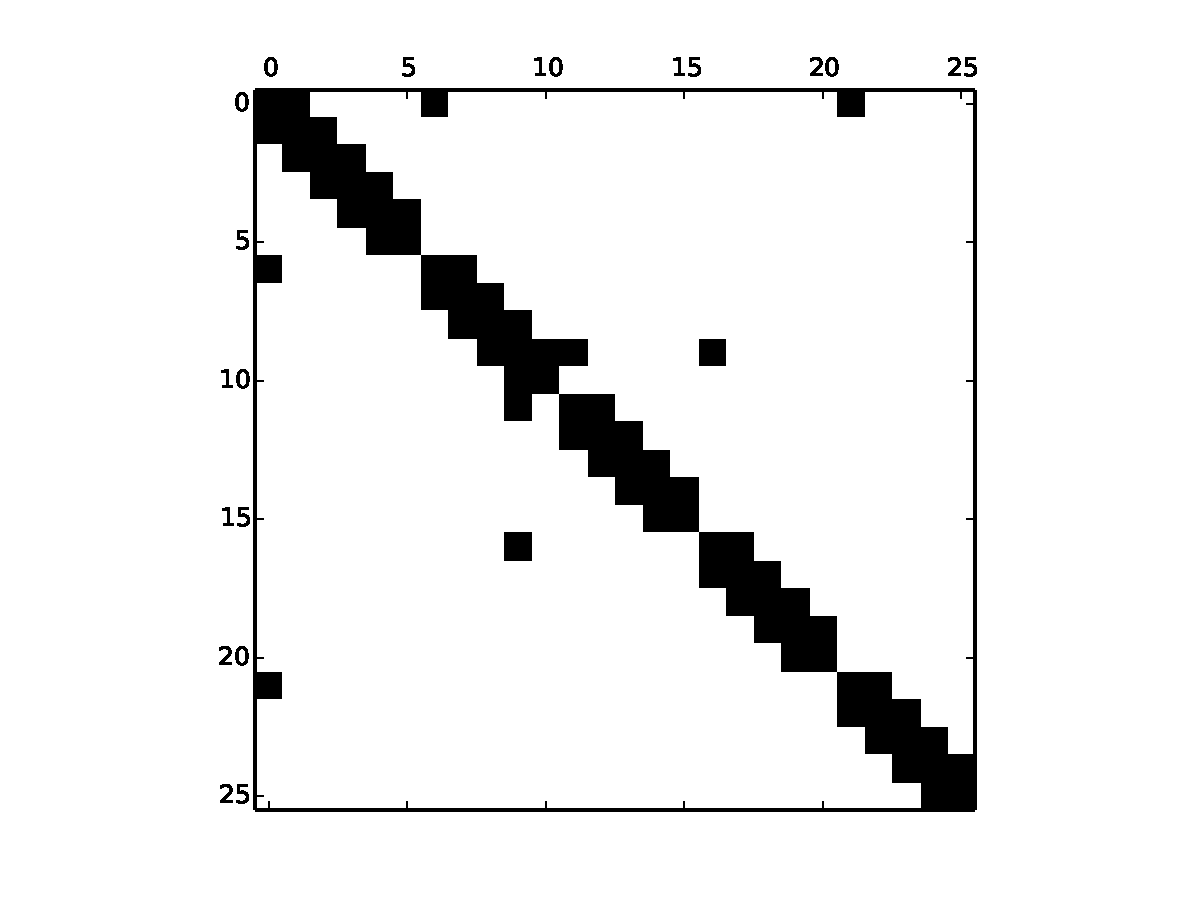
\includegraphics[width=0.5\textwidth]{./images/sparsity.pdf}
\caption{Sparsity pattern of the matrix corresponding to the tree numbering in \fig{fig:tree}.}
\label{fig:sparsity}
\end{figure}


The linear systems that arise from the discretization of the branching cable equation can be solved very efficiently, in linear $O(N)$ time, using an algorithm that is equivalent to the Thomas algorithm for solving tri-diagonal systems. This algorithm, called Hines algorithm, proceeds by eliminating the nonzero entries in the upper triangle of $A$. Recall the matrix property that there is only one non-zero value in each column of the upper triangle
 at $A_{ki}$, which is stored in $a_i$.
\begin{equation}
\left(
        \begin{array}{ccc}
            A_{kk} & \dots      & A_{ki} \\
        \vdots     & \ddots     & \mathbf{0} \\
            A_{ik} & \mathbf{0} & A_{ii}
        \end{array}
\right)
\text{which is stored as:}
\left(
        \begin{array}{ccc}
            d_k & \dots      & a_i \\
        \vdots  & \ddots     & \mathbf{0} \\
            b_i & \mathbf{0} & d_i
        \end{array}
\right)
\end{equation}
The value $a_i$ and can be zeroed out with a row operation $\text{row}_k -= a_i/d_i\cdot\text{row}_i$. In practice the value of $a_i$ is not changed, and only the diagonal entry has to be modified $d_k -= a_i/d_i\cdot b_i$. The forward substitution is then used to determine the solution. The forward and backward substitution are implemented in Julia in \ap{appendix:hinessource}.

%%%%%%%%%%%%%%%%%%%%%%%%%%%%%%%%%%%%%%%%%%%%%%%%%%%%%%%%%%%%%%
\subsection{Implementation of a time step}
%%%%%%%%%%%%%%%%%%%%%%%%%%%%%%%%%%%%%%%%%%%%%%%%%%%%%%%%%%%%%%
In this section the implementation of the code that forms and solves the matrix, which accounts for 99\% of the time to solution will be described. The algorithm themselves are quite simple, however their implementation is very difficult to understand. To make it easier to understand to understand implementation, the core routines have been rewritten in a high-level pseudo code similar to Julia.

An example of the pseudo code represents the following C code
\begin{shaded}
\begin{lstlisting} [breaklines=true]
for (tml = _nt->tml; tml; tml = tml->next)
  if (memb_func[tml->index].current) {
    mod_f_t s = memb_func[tml->index].current;
    (*s)(_nt, tml->ml, tml->index);
  }
\end{lstlisting}
\end{shaded}
\noindent as
\begin{shaded}
\begin{lstlisting} [language=julia,breaklines=true]
for mechanism in thread.mechanisms
  mechanism.current(thread, mechanism.data)
end
\end{lstlisting}
\end{shaded}
\noindent The pseudo code should run in julia with very little modification (a similar level of clarity would be possible with well-designed C+11 code).

The inner part of each time step is implemented in the function \lst{nrn_fixed_step_thread()}, in \file{nrnoc/fadvance_core.c}. The routine takes as its argument a pointer to a struct of type \lst{NtnThread}, see \fig{lst:NrnThread}, which holds state relating to a set of cells to be integrated in time.
\begin{shaded}
\lstinputlisting [language=julia,breaklines=true] {./code/fixed_step_thread.jl}
\end{shaded}

A breakdown of wall time for the steps in \lst{nrn_fixed_step()} is given in \fig{fig:calltree}. Some of the routines listed here have less than 1\% of wall time (including the linear system solve in \lst{nrn_solve_minimal()}), however they are discussed below because they access they have implementation details that will influence the implementation on many-core architectures (e.g. GPU and MIC).

%%%%%%%%%%%%%%%%%%%%%%%%%%%%%%%%%%%%%%%%%%%%%%%%%%%%%%%%%%%%%%
\subsubsection{Building matrix and RHS: \lst{setup_tree_matrix()}}
%%%%%%%%%%%%%%%%%%%%%%%%%%%%%%%%%%%%%%%%%%%%%%%%%%%%%%%%%%%%%%
The function \lst{setup_tree_matrix()} generates the diagonal, the $d_i$ values, and the RHS vector. These tasks are performed in two separate routines, \lst{nrn_lhs()} and \lst{nrn_rhs()}.
\begin{shaded}
\lstinputlisting [language=julia,breaklines=true] {./code/setup_tree_matrix.jl}
\end{shaded}

Points
\begin{itemize}
\item
    The array \lst{p} is an index array containing the parent node indexes.
\item
    The arrays \lst{VEC_*} correspond to the vectors $\vv{a}, \vv{b}, \vv{d}, \vv{v}, \vv{r}$ that define the linear system.
\item
    Each thread has multiple cells, each with their own tree representation. The cells are packed together, with the root node of each cell placed first in the list of all nodes, hence the definition of \lst{child_nodes} excluding indexes $1:ncells$.
\item
    Nearly all (i.e. 99\%) of the time in these two routines is spent in the calls to the \lst{mechanism.current()} and \lst{mechanism.jacob()} routines.
\item
    The matrix updates still must be considered, because there are potential race conditions in a multi-threaded/GPU implementation. For example the statement \lst{VEC_RHS[p[i]] += dv * VEC_A[i]} will lead to a race condition if two threads with the same parent node try to update the RHS vector at the same time.
\end{itemize}

The \lst{mechanism.current()} and \lst{mechanism.jacob()} routines are defined in the \file{/mech/cfiles} path, and are automatically generated from Neuron hoc DSL. \fig{fig:calltree} shows that all of the computational work in the \neuron benchmark used in this report is performed by functions from the hoc layer.

%%%%%%%%%%%%%%%%%%%%%%%%%%%%%%%%%%%%%%%%%%%%%%%%%%%%%%%%%%%%%%
\section{Benchmarking}
%%%%%%%%%%%%%%%%%%%%%%%%%%%%%%%%%%%%%%%%%%%%%%%%%%%%%%%%%%%%%%
%-------------------------------------------------------------------------------
\begin{table}[htp!]
    \centering
%-------------------------------------------------------------------------------
\begin{tabular}{l|l|rrrrr}
\multirow{2}{*}{}
& cells-per-core  &    1  & 2     & 4     & 8  & 16  \\
& cells-per-node  &    8  & 16    & 32    & 64 & 128 \\
\hline
\multirow{8}{*}{nodes}
&1                & 390.8 & 383.6 & 381.6 & 380.5 & 381.3\\
&2                & 390.9 & 385.1 & 384.0 & 385.3 & 382.5\\
&4                & 394.8 & 392.7 & 389.9 & \textcolor{blue}{194.1} & 382.6\\
&8                & 400.4 & 392.8 & 385.9 & 382.7 & 381.0\\
&16               & 401.9 & 394.3 & 388.6 & 384.2 & 381.8\\
&32               & 401.7 & 393.6 & 387.0 & 383.8 & \textcolor{red}{DNF}\\
&64               & 403.0 & 395.7 & 390.0 & 385.4 & 382.3 \\
&128              & 411.0 & 396.1 & 390.4 & 385.5 & 378.7 \\
&256              & 411.4 & 397.0 & 390.7 & \textcolor{blue}{195.5} & 374.9\\
&512              & 413.5 & 396.8 & 389.2 & 377.7 & --\\
%\hline
\end{tabular}

%-------------------------------------------------------------------------------
\label{tbl:test2scaling}
\caption{Wall time for TEST2 as both the number of nodes and cells-per-node are varied. Each test always use 8 cores/MPI ranks per-node. The times in \textcolor{blue}{blue} indicate unexplained timings, and those marked \textcolor{red}{DNF} did not finish due to memory restrictions (it is not possible to run with more than 16 cells per node due to memory restrictions.)}
\end{table}
%-------------------------------------------------------------------------------

\todo{describe adding Papi counters to instrument parts of code. Show basic timing results in \fig{fig:calltree}.}

\begin{figure}[htp!]
\centering
\includegraphics[width=\textwidth]{./images/calltree.pdf}
\caption{Calltree and percentage of wall time contribution for the main computational algorithm. Branches marked in blue indicate a significant contribution to wall time.}
\label{fig:calltree}
\end{figure}

%%%%%%%%%%%%%%%%%%%%%%%%%%%%%%%%%%%%%%%%%%%%%%%%%%%%%%%%%%%%%%%%%%%%%%%%%%%%%%%%%%%
%%%%%%%%%%%%%%%%%%%%%%%%%%%%%%%%%%%%%%%%%%%%%%%%%%%%%%%%%%%%%%%%%%%%%%%%%%%%%%%%%%%
\newpage
\appendix
%%%%%%%%%%%%%%%%%%%%%%%%%%%%%%%%%%%%%%%%%%%%%%%%%%%%%%%%%%%%%%%%%%%%%%%%%%%%%%%%%%%
%%%%%%%%%%%%%%%%%%%%%%%%%%%%%%%%%%%%%%%%%%%%%%%%%%%%%%%%%%%%%%%%%%%%%%%%%%%%%%%%%%%

%%%%%%%%%%%%%%%%%%%%%%%%%%%%%%%%%%%%%%%%%%%%%%%%%%%%%%%%%%%%%%%%%%%%%%%%%%%%%%%%%%%
\newpage
\section{Source code for constructing a tree}
%%%%%%%%%%%%%%%%%%%%%%%%%%%%%%%%%%%%%%%%%%%%%%%%%%%%%%%%%%%%%%%%%%%%%%%%%%%%%%%%%%%
\label{appendix:treesource}
\todo{describe code}
\begin{shaded}
\lstinputlisting [language=julia,breaklines=true] {./code/tree.jl}
\end{shaded}

%%%%%%%%%%%%%%%%%%%%%%%%%%%%%%%%%%%%%%%%%%%%%%%%%%%%%%%%%%%%%%%%%%%%%%%%%%%%%%%%%%%
\newpage
\section{Source code for Hines algorithm}
%%%%%%%%%%%%%%%%%%%%%%%%%%%%%%%%%%%%%%%%%%%%%%%%%%%%%%%%%%%%%%%%%%%%%%%%%%%%%%%%%%%
\label{appendix:hinessource}
\todo{describe code}
\begin{shaded}
\lstinputlisting [language=julia,breaklines=true] {./code/hines.jl}
\end{shaded}

\end{document}
